%!TEX program = xelatex

\documentclass[onecolumn,a4paper,10pt]{article}

\usepackage[ boldfont,slantfont]{xeCJK}  %设定支持中文
\usepackage{multicol}

\graphicspath{{figures/}}    %设置放置图片的文件夹

\linespread{1.2}     %设置行间距的命令

\setmainfont{Times New Roman}

%for windows fonts
%\setCJKmainfont[BoldFont={SimHei},ItalicFont={KaiTi}]{SimSun}
%\setsansfont{SimHei}
%
%\setCJKfamilyfont{song}{SimSun}
%\setCJKfamilyfont{kai}{KaiTi}
%\setCJKfamilyfont{hei}{SimHei}
%\setCJKfamilyfont{yao}{FZYaoTi}
%
%\newcommand\song{\CJKfamily{song}}
%\newcommand\kai{\CJKfamily{kai}}
%\newcommand\hei{\CJKfamily{hei}}
%\newcommand\yao{\CJKfamily{yao}}

\setCJKmainfont[BoldFont={STXihei},ItalicFont={STKaiti}]{STSong}
\setsansfont{STXihei}

\setCJKfamilyfont{song}{STSong}
\setCJKfamilyfont{kai}{STKaiti}
\setCJKfamilyfont{hei}{STXihei}
%\setCJKfamilyfont{yao}{FZYaoTi}

\newcommand\song{\CJKfamily{song}}
\newcommand\kai{\CJKfamily{kai}}
\newcommand\hei{\CJKfamily{hei}}
%\newcommand\yao{\CJKfamily{yao}}

\newcommand{\erhao}{\fontsize{22pt}{\baselineskip}\selectfont}
\newcommand{\xiaoerhao}{\fontsize{18pt}{\baselineskip}\selectfont}
\newcommand{\sanhao}{\fontsize{16pt}{\baselineskip}\selectfont}
\newcommand{\xiaosanhao}{\fontsize{15pt}{\baselineskip}\selectfont}
\newcommand{\sihao}{\fontsize{14pt}{\baselineskip}\selectfont}
\newcommand{\xiaosihao}{\fontsize{12pt}{\baselineskip}\selectfont}
\newcommand{\wuhao}{\fontsize{10.5pt}{\baselineskip}\selectfont}
\newcommand{\xiaowuhao}{\fontsize{9pt}{\baselineskip}\selectfont}
\newcommand{\liuhao}{\fontsize{7.5pt}{\baselineskip}\selectfont}

%%%段落首行缩进两个字
\makeatletter
\let\@afterindentfalse\@afterindenttrue
\@afterindenttrue
\makeatother
\setlength{\parindent}{2em}%中文缩进两个汉字位

%%%%%%%%%% 定理类环境的定义 %%%%%%%%%%
%% 必须在导入中文环境之后
\newtheorem{example}{例}             % 整体编号
\newtheorem{algorithm}{算法}
\newtheorem{theorem}{定理}[section]  % 按 section 编号
\newtheorem{definition}{定义}
\newtheorem{axiom}{公理}
\newtheorem{property}{性质}
\newtheorem{proposition}{命题}
\newtheorem{lemma}{引理}
\newtheorem{corollary}{推论}
\newtheorem{remark}{注解}
\newtheorem{condition}{条件}
\newtheorem{conclusion}{结论}
\newtheorem{assumption}{假设}

%%%%%%%%%% 一些重定义 %%%%%%%%%%
%% 必须在导入中文环境之后
\renewcommand{\contentsname}{目录}     % 将Contents改为目录
\renewcommand{\abstractname}{摘\ \ 要} % 将Abstract改为摘要
\renewcommand{\refname}{参考文献}      % 将References改为参考文献
\renewcommand{\indexname}{索引}
\renewcommand{\figurename}{图}
\renewcommand{\tablename}{表}
\renewcommand{\appendixname}{附录}
%\renewcommand{\proofname}{证明}
\renewcommand{\algorithm}{算法}

%%%%%%%%%%%%%%%%%%%%%%%%%%%%%%%%%%%%%%%%%%%%%%%%%%%%%%%%%%%%%%%%
%  packages
%    这部分声明需要用到的包
%%%%%%%%%%%%%%%%%%%%%%%%%%%%%%%%%%%%%%%%%%%%%%%%%%%%%%%%%%%%%%%%
\usepackage{graphicx}    % EPS 图片支持
\usepackage{indentfirst} % 中文段落首行缩进
\usepackage{bm}          % 公式中的粗体字符(用命令\boldsymbol)
\usepackage{graphics}	%让文档支持图片
\usepackage{amsmath}	%ams可以让文档支持数学公式

\usepackage{float}
\usepackage{fontspec,xunicode,xltxtra}
\usepackage{hyperref}	%让文档支持超链接
\usepackage{booktabs}	%让文档支持三线表格
\usepackage{amsfonts}
\usepackage{amssymb}
\usepackage{color}
\usepackage{graphicx,psfrag}
\usepackage{epsfig}
\usepackage{verbatim}
\usepackage{picins}
\usepackage{multirow}
\usepackage{listings} 
\usepackage{xcolor}
\usepackage[titletoc]{appendix} %附件支持


%%%%%%%%%%%%%%%%%%%%%%%%%%%%%%%%%%%%%%%%%%%%%%%%%%%%%%%%%%%%%%%%
%  lengths
%    下面的命令重定义页面边距,使其符合中文刊物习惯。
%%%%%%%%%%%%%%%%%%%%%%%%%%%%%%%%%%%%%%%%%%%%%%%%%%%%%%%%%%%%%%%%
\addtolength{\topmargin}{-54pt}
\setlength{\oddsidemargin}{0.63cm}  % 3.17cm - 1 inch
\setlength{\evensidemargin}{\oddsidemargin}
\setlength{\textwidth}{14.66cm}
\setlength{\textheight}{24.00cm}    % 24.62
\begin{document}
%%%%%%%%%%%%%%%%%%%%%%%%%%%%%%%%%%%%%%%%%%%%%%%%%%%%%%%%%%%%%%%%
%  定义标题格式,包括title,author,affiliation,email等。
%  在任何用到中文的地方,用\begin{CJK} ... \end{CJK}将其括起来。
%%%%%%%%%%%%%%%%%%%%%%%%%%%%%%%%%%%%%%%%%%%%%%%%%%%%%%%%%%%%%%%%
\title{\hei{蒸发冷却方案比较 }}
\author{肖波\footnote{xbustc@gmail.com}~~~~~~
\\[8pt]
\xiaowuhao 合肥微尺度物质科学国家实验室,安徽~~合肥~~230026\\[4pt]
}
%\date{\today}  % 这一行用来去掉默认的日期显示
\date{\today}  
%%%%%%%%%%%%%%%%%%%%%%%%%%%%%%%%%%%%%%%%%%%%%%%%%%%%%%%%%%%%%%%%
%  自定义命令
%%%%%%%%%%%%%%%%%%%%%%%%%%%%%%%%%%%%%%%%%%%%%%%%%%%%%%%%%%%%%%%%
% 此行使文献引用以上标形式显示
%\newcommand{\super}[1]{\textsuperscript{\cite{#1}}}
%%%%%%%%%%%%%%%%%%%%%%%%%%%%%%%%%%%%%%%%%%%%%%%%%%%%%%%%%%%%%%%%
%  显示title,并设页码为空(按杂志社要求)
%%%%%%%%%%%%%%%%%%%%%%%%%%%%%%%%%%%%%%%%%%%%%%%%%%%%%%%%%%%%%%%%
\maketitle  
%\pagestyle{empty} \thispagestyle{empty}
\vspace{-20pt}

%%%%%%%%%%%%%%%%%%%%%%%%%%%%%%%%%%%%%%%%%%%%%%%%%%%%%%%%%%%%%%%%
%  中文摘要
%%%%%%%%%%%%%%%%%%%%%%%%%%%%%%%%%%%%%%%%%%%%%%%%%%%%%%%%%%%%%%%%

%\begin{center}
%\parbox{\textwidth}{
%%\rule{2em}{0pt}
%\hei{摘要:}\song{在超冷原子相关的实验中,磁场的稳定性会极大的影响原子的退相干时间,因此,在大部分的超冷原子实验中都会配备PID反馈系统用以稳定原子的偏置磁场,延长相干时间。本方案基于海德堡光晶格实验室目前的方案,用以稳定原子的任意方向偏置磁场。}\\[5pt]
%\hei{关键词:}\song{很关键;很关键;非常关键}
%\\[5pt]
%}
%\end{center}



\iffalse
%%%%%%%%%%%%%%%%%%%%%%%%%%%%%%%%%%%%%%%%%%%%%%%%%%%%%%%%%%%%%%%%
%  英文摘要
%%%%%%%%%%%%%%%%%%%%%%%%%%%%%%%%%%%%%%%%%%%%%%%%%%%%%%%%%%%%%%%%
\begin{center}
\sihao{\textbf{A \LaTeX{} Template for Chinese Reports}}\\[7pt]
\normalsize
Weiyong Zhang~~~~~~
\\[7pt]
\xiaowuhao Hefei National Laboratory for Physical Sciences at the Microscale, HeFei, AnHui, 230026\\[10pt]
\end{center}
\begin{center}
\parbox{\textwidth}{
\textbf{Abstract:} This is a \LaTeX{} template used for writting documents in Chinese form.\\[4pt]
\textbf{Keywords:} Key; Key; the Key
}
\end{center}
\fi

\begin{table}[H]
\small
\centering
\caption{各组蒸发冷却条件和结果对比}
\label{tab:chap04-01}
\begin{tabular}{l|l|l|l|l|l|l|l}
\hline
Group & Initial T & Initial PSD& Initial N & Final PSD & Final N & RF time & Dipole trap time  \\
\hline
I.B. Spielman & $190\mu K/29\mu K$ &$5*10^{-7} /1.79*10^{-4}$& $9*10^8/8*10^7$& >2.612&$1.8*10^6$&2.9 s&3 s+4s\\
\hline
Cheng Chin/Cs&$0.47 \mu K$&0.0445&$1.9*10^6$&2.6&$5*10^5$&&4s/1.8s\\
\hline
Yong P. Chen&$60\mu K$&$2.59*10^{-4}$&$5*10^5$&2.6&$4.9*10^4$&&4.35s\\
\hline
Heidelberg&$130 \mu K/26\mu K$&$5*10^{-7}/1.83*10^{-4}$&$5*10^8/6*10^7$&3.4&$2*10^5$&2s&0.5s+4s\\
\hline
\end{tabular}
\end{table}

\section{J.V Porto, I.B. Spielman\cite{mc1}}

该组使用了一个磁阱和一个dipole trap结合的方法,光阱的中心在磁场中心下方一个束腰左右的位置,以减小Majorana Loss,开始的时候使用RF 蒸发方法2s内将原子冷却到30 $\mu K$左右,这个时候重力和磁场的力抵消,单独光阱囚禁铷原子用4s做蒸发冷却达到BEC。
\begin{figure}[htbp]
\centering
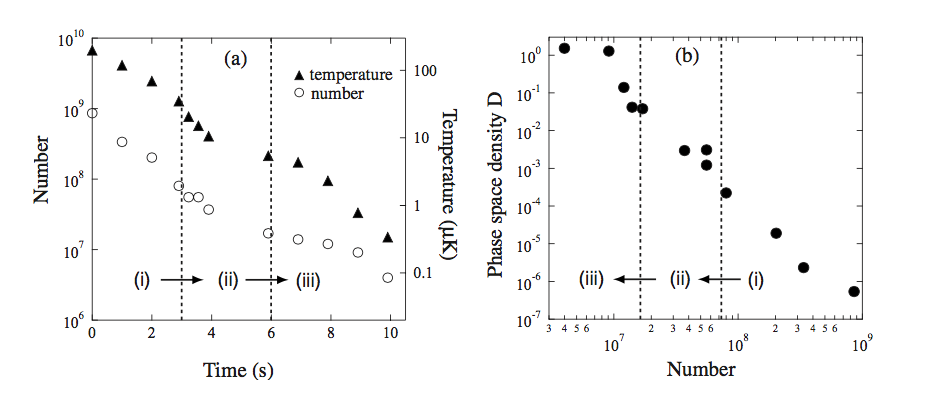
\includegraphics[width=1\textwidth]{Spielman}
\caption{PSD and Number}
\label{fig1:Spielman}
\end{figure}


\section{Cheng Chin\cite{mc2}}

水平面的两束交叉光,交叉光中心和磁场中心重合,交叉光的存在使得势阱在三个方向上对原子都有很好的束缚,同时在铯原子处用亥姆霍兹线圈产生了一个均匀的20.8G用以消除三体碰撞损失。在实际蒸发过程中,只需要将梯度磁场增大使得高能原子在重力作用下逃出势阱,达到蒸发的效果,实验者尝试在1s内达到BEC,最终原子数较少($4*10^4$)。使用4s的时间能实现Runaway 的蒸发,1.8s也能达到BEC,但是这个快速是建立在起始PSD在$4*10^{-2}$左右的基础上。
\begin{figure}[H]
\centering
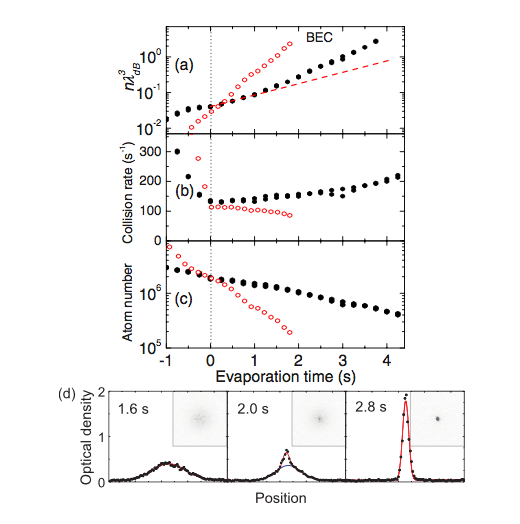
\includegraphics[width=0.7\textwidth]{ChengChin}
\caption{PSD and Number}
\label{fig2:ChengChin}
\end{figure}

\section{Yong P. Chen\cite{mc3}}
这个方案完全是在光阱中实现的,在整个过程中,两束交叉光中心有个偏差,通过调节光强的大小,进一步可以调节平衡位置和对应的阱频率,实现蒸发,整个方案有理论模型模拟,找出了截断常数和频率与势阱深度的关系指数的优化值,在这个优化参数下,蒸发效率可以高达3.95。该组在实现BEC的时候,规管显示的真空腔的气压高达$1*10^{-9}  Torr$,这个跟我们目前的真空情况很类似,不过作者也提到,对势阱装载的测量显示真空度应该比显示的要好。
\begin{figure}[H]
\centering
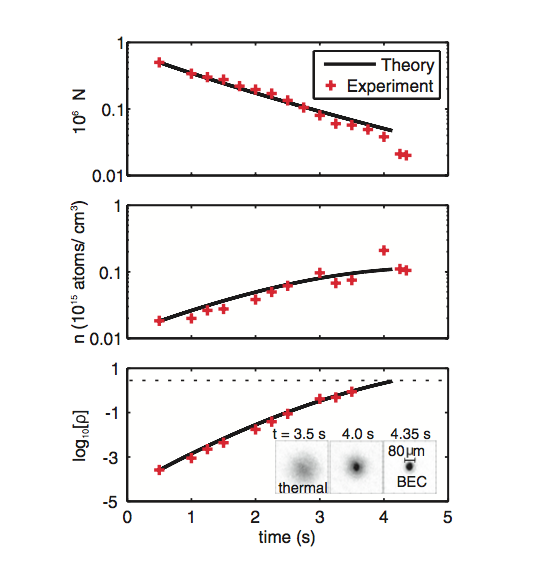
\includegraphics[width=0.7\textwidth]{ChenP}
\caption{PSD and Number}
\label{fig3:ChenP}
\end{figure}

\section{Heidelberg}
方案基本参考Spielman组的装载和射频蒸发,磁阱向光阱装载的的时间只有0.5s,会不会是因为磁场关断比使用金属腔的Spielman组快所以可以快速装载?并且为了获得更快的蒸发速度,采用了交叉光阱以提高阱频率,提高碰撞率。

\begin{figure}[H]
\centering
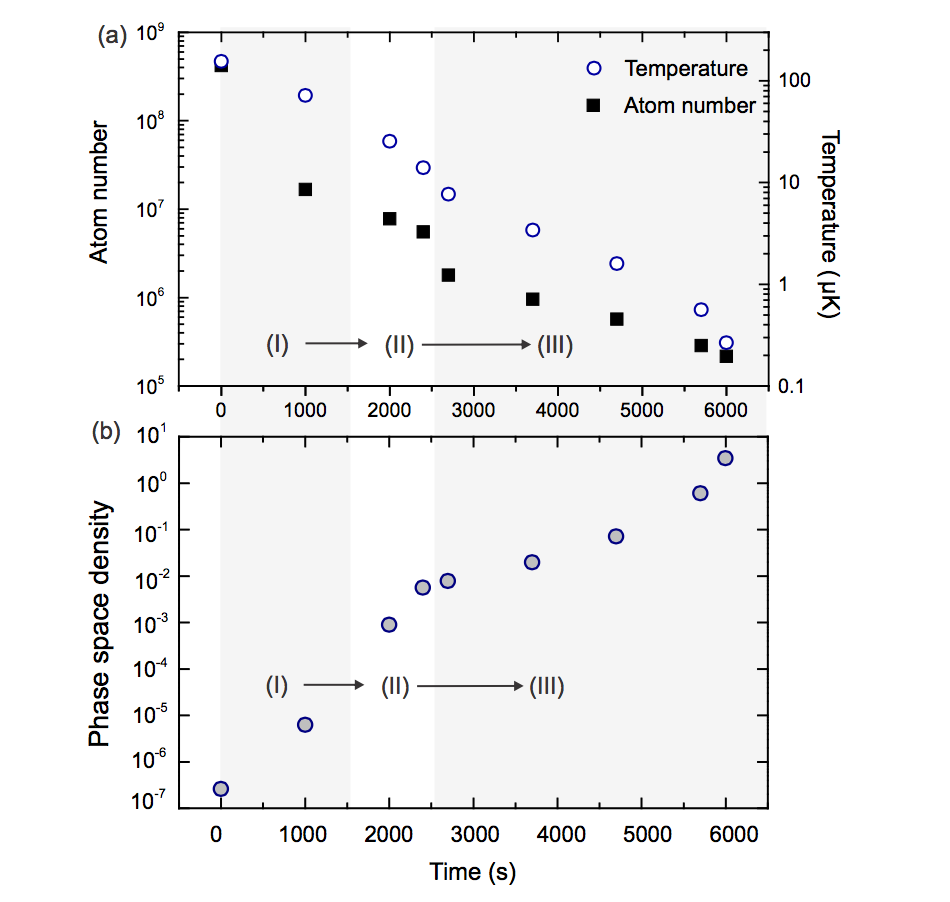
\includegraphics[width=1\textwidth]{YangBing}
\caption{PSD and Number}
\label{fig4:YangBing}
\end{figure}


%\section{参考文献}
%%%%%%%%%%%%%%%%%%%%%%%%%%%%%%%%%%%%%%%%%%%%%%%%%%%%%%%%%%%%%%%%
%  参考文献
%%%%%%%%%%%%%%%%%%%%%%%%%%%%%%%%%%%%%%%%%%%%%%%%%%%%%%%%%%%%%%%%
\small
\begin{thebibliography}{99}
\setlength{\itemsep}{0pt}
\setlength{\parskip}{0pt}  %段落之间的竖直距离
\bibitem{mc1} Lin Y J, Perry A R, Compton R L, et al. Rapid production of $^{87}$Rb Bose-Einstein condensates in a combined magnetic and optical potential[J]. Physical Review A, 2009, 79(6): 063631.

\bibitem{mc2} Hung C L, Zhang X, Gemelke N, et al. Accelerating evaporative cooling of atoms into Bose-Einstein condensation in optical traps[J]. Physical Review A, 2008, 78(1): 011604.

\bibitem{mc3}Olson A J, Niffenegger R J, Chen Y P. Optimizing the efficiency of evaporative cooling in optical dipole traps[J]. Physical Review A, 2013, 87(5): 053613.
\end{thebibliography}





\end{document}

